\documentclass[11pt]{article}
\usepackage[margin=1in]{geometry}
\usepackage[T1]{fontenc}
\usepackage{lmodern}
\usepackage{amsmath,amssymb}
\usepackage{booktabs}
\usepackage{graphicx}
\usepackage{xcolor}
\usepackage[numbers,sort&compress]{natbib}
\usepackage[hidelinks]{hyperref}
\usepackage{caption}
\captionsetup{font=small,labelfont=bf}

% Numbers still waiting on runs are marked in red; remove before submission.
\newcommand{\pending}[1]{\textcolor{red}{[#1]}}
\newcommand{\dc}{$\Delta$Context}

\title{\dc: Online Semantic-Change Segmentation for\\Topic-Structured Conversational Memory}
\author{\pending{Author names}\\\pending{Affiliation}\\\texttt{\pending{email}}}
\date{}

\begin{document}
\maketitle

\begin{abstract}
A long-running chat assistant must decide which part of an ever-growing
conversation history to place in a bounded context window. We treat this as a
\emph{storage} problem: if the history is stored as topic segments as it
arrives, returning to an earlier topic and retrieving from it become cheap. We
present \dc{}, an online segmenter that tracks how far a windowed embedding of
the conversation has moved from the state at the current topic's start, and
places each boundary at the sharpest single-turn semantic jump. On
LongMemEval-S, \dc{} is the most accurate of the segmenters we compare,
including offline semantic chunking and TextTiling (Pk 0.099 vs.\ 0.125--0.212;
boundary F1 0.84 vs.\ at most 0.78), while deciding turn by turn. As the index
of a topic-first store it returns the right topic first for 75\% of questions
and keeps 93\% of a full scan's evidence recall while searching 17\% of the
turns; as the store grows to $\sim$20K turns it stays close to an oracle
segmentation while fixed-size chunks and semantic chunking fall behind. We
also show that a widely used LoCoMo evaluation setup mis-scores 38\% of its
probes and release corrected scoring. Finally we report negative results:
topic-first retrieval does not beat scanning every turn on recall or
end-to-end answer quality, and on a single history its retrieval advantage over
other semantic segmenters is small and not statistically significant.
\end{abstract}

% ---------------------------------------------------------------------------
\section{Introduction}

Conversational assistants that persist across sessions accumulate histories
far longer than any practical prompt: the LoCoMo conversations run to 30K
tokens \citep{maharana2024locomo} and each LongMemEval-S question comes with
$\sim$115K tokens of chat \citep{wu2025longmemeval}. Even with long-context
models, placing everything in the prompt is costly and models use long inputs
unevenly \citep{liu2024lost}. A \emph{context management policy} therefore
chooses, under a token budget, which past turns the model sees. Common choices
are truncation to the most recent turns, summarisation of dropped turns, and
retrieval of turns similar to the current question
\citep{lewis2020rag,packer2023memgpt,zhong2024memorybank,chhikara2025mem0}.

Retrieval over individual turns ignores a property of real conversations: they
move between topics, and questions often return to one. We ask whether storing
a chat as \emph{topic segments}, found online as the chat unfolds, makes two
operations easier: \emph{topic switching} (restoring the context of a topic
the user returns to) and \emph{retrieval} (searching a few topics instead of
every turn). This requires a segmenter that works incrementally, without
seeing the rest of the history, and that places boundaries precisely enough
for segment centroids to stay pure.

\paragraph{Contributions.}
\begin{enumerate}
  \item \dc{}, an online topic segmenter for conversations built on the
  displacement of a windowed embedding state from the current topic's
  reference state, with \emph{boundary localisation} that corrects the window's
  detection lag (\S\ref{sec:method}). It is the most accurate segmenter we
  test on LongMemEval-S, ahead of two offline methods, and both of its design
  choices are necessary (\S\ref{sec:seg}).
  \item A topic-first store on these segments, evaluated for topic switching
  and retrieval cost, including a scaling study to $\sim$20K-turn stores
  (\S\ref{sec:store}--\ref{sec:scaling}).
  \item A corrected LoCoMo evaluation: the common setup grades adversarial
  questions against their trap answers and hides session dates, mis-scoring
  38\% of probes for every policy (\S\ref{sec:setup}).
  \item A controlled benchmark (\textsc{ContextBench}) in which the model,
  prompt, tokenizer and embedder are fixed and only the policy varies, and an
  honest account of where topic-structured memory does \emph{not} help
  (\S\ref{sec:negative}).
\end{enumerate}

% ---------------------------------------------------------------------------
\section{Related Work}

\paragraph{Conversational memory.} Memory systems for LLM agents page content
in and out of the context \citep{packer2023memgpt}, maintain summaries or
memory banks \citep{zhong2024memorybank,park2023generative}, or extract
structured facts \citep{chhikara2025mem0}. LoCoMo \citep{maharana2024locomo}
and LongMemEval \citep{wu2025longmemeval} benchmark long-term conversational
memory; we use both and correct a common LoCoMo scoring practice.

\paragraph{Retrieval granularity.} Retrieval-augmented generation
\citep{lewis2020rag} depends on how text is chunked. Hierarchical indexes
summarise chunks into a tree \citep{sarthi2024raptor}; RAG toolkits offer
``semantic chunking'' that splits where consecutive sentence embeddings
diverge \citep{langchain2024semanticchunker}. These operate offline on a
complete document; \dc{} segments a conversation as it arrives.

\paragraph{Topic segmentation.} TextTiling \citep{hearst1997texttiling} and
C99 \citep{choi2000c99} segment text by lexical cohesion; Pk
\citep{beeferman1999statistical} and WindowDiff \citep{pevzner2002critique} are
the standard metrics. Dialogue topic segmentation has been studied with
utterance-pair coherence \citep{xing2021improving}. We compare against
embedding-based TextTiling and semantic chunking, and evaluate segmentation
both intrinsically and by its effect on retrieval.

% ---------------------------------------------------------------------------
\section{Method}
\label{sec:method}

\subsection{Problem}
A conversation is a sequence of turns $u_1, u_2, \dots$. At question time,
a policy selects a subset of past turns whose rendered length is at most a
budget $B$ tokens; a fixed language model answers from the selected turns.

\subsection{Online segmentation}
Let $e_t$ be the L2-normalised embedding of turn $u_t$. \dc{} maintains a
windowed state $C_t = \frac{1}{w}\sum_{i=t-w+1}^{t} e_i$ ($w = 3$) and the
state $C_{\mathrm{ref}}$ recorded at the last checkpoint. Its change signal is
the \emph{displacement} from the current topic's reference,
\begin{equation}
  A_t = 1 - \cos(C_{\mathrm{ref}}, C_t),
\end{equation}
and a checkpoint fires when $A_t \ge \tau$ and at least $g$ turns have passed
since the previous one ($g = 3$). Displacement measures net movement away from
where the topic started, so it rises sharply at a topic switch and stays low
during on-topic chatter; the path-length alternative
$A_t = \sum \delta_i$, with $\delta_i = 1 - \cos(C_{i-1}, C_i)$ summed since
the last checkpoint, accumulates ordinary chatter and fires on volume rather
than on switches (\S\ref{sec:seg}).

\paragraph{Boundary localisation.} Because $C_t$ averages $w$ turns, it
crosses $\tau$ only once most of the window holds the new topic, so
checkpoints fire $w - 1$ turns late. \dc{} therefore starts the new segment at
\begin{equation}
  s = \operatorname*{arg\,max}_{t-w+1 \le i \le t}\; \bigl(1 - \cos(e_{i-1}, e_i)\bigr),
\end{equation}
the sharpest single-turn jump within the window that triggered the checkpoint.
Each segment is indexed by the centroid of its turn embeddings. Per turn, the
cost is one embedding and $O(w)$ vector operations; nothing is recomputed.

\subsection{Topic-first retrieval}
Given a question with embedding $q$, \dc{} (i) ranks segments by
$\cos(q, \text{centroid})$ and keeps the top $k$; (ii) ranks only the turns
inside those segments by $\cos(q, e_t)$; and (iii) fills the budget greedily
in that order, skipping turns that do not fit, continuing with the remaining
turns by similarity if the selected topics are exhausted. Selected turns are
rendered chronologically with their session dates. A query costs
$|\text{segments}| + |\text{turns in the top-}k\text{ segments}|$ similarity
computations instead of one per turn.

% ---------------------------------------------------------------------------
\section{Experimental Setup}
\label{sec:setup}

\paragraph{Benchmark.} In \textsc{ContextBench} the policy is the only
variable: the generator, prompt, tokenizer (which also measures every budget),
embedder and decoding are shared. Generator: Qwen2.5-3B-Instruct
\citep{qwen2024qwen25} in bfloat16 with greedy decoding; embedder:
all-MiniLM-L6-v2 \citep{wang2020minilm,reimers2019sbert}.

\paragraph{Datasets.} \emph{LongMemEval-S} \citep{wu2025longmemeval}: 500
questions, each with its own history of $\sim$48 sessions (median 491 turns)
on mostly unrelated topics; 479 carry turn-level evidence labels and 30 are
abstention questions. Its sessions are topics, so session boundaries serve as
the segmentation reference. \emph{LoCoMo} \citep{maharana2024locomo}: 10
two-person conversations (369--689 turns) with 1,986 QA probes; its sessions
are days of one continuing conversation, not topics.

\paragraph{Corrected LoCoMo scoring.} The common setup has two problems that
affect every policy equally. (i) The 446 adversarial probes (22\%) ask about
something the conversation never says, typically a fact re-attributed to the
other speaker; their \texttt{adversarial\_answer} field is the \emph{trap}
answer, and grading F1 against it rewards being fooled. We score them on
abstention, as LoCoMo's own evaluation does, and report them separately; the
headline metrics cover the 1,540 answerable probes. (ii) Session dates are
loaded but never shown, so the 321 temporal probes (16\%) are unanswerable; we
prefix each transcript line with its session date and count those tokens
against the budget. We also use a short-answer prompt, without which exact
match was 0 for every probe.

\paragraph{Baselines.} Sliding window (newest turns); an extractive summary of
dropped turns plus the newest turns; RAG over turns with half the budget for
the newest turns (the original configuration) and with the whole budget for
retrieval (full scan); and topic-first stores identical to \dc{} except for
the segmentation: fixed-size chunks, an online adjacent-turn threshold
(cut where $1-\cos(e_{t-1},e_t) > \theta$), offline semantic chunking (cut where
the consecutive distance exceeds its $p$-th percentile in the history), offline
TextTiling over embeddings \citep{hearst1997texttiling}, and the session
boundaries themselves (an oracle). On LoCoMo the full conversation fits
Qwen's 32K window and gives an upper bound.

\paragraph{Metrics.} \emph{Segmentation}: Pk, WindowDiff, and boundary
precision/recall/F1 with one-to-one matching at tolerance 0 and $\pm 1$ turn.
\emph{Topic store}: topic hit@$k$ (an evidence turn lies in one of the $k$ best
topics); topic recall (evidence turns that are both selected and inside the
searched topics); and the share of a full scan's comparisons. \emph{Selection}:
evidence recall, the share of labelled evidence turns in the context.
\emph{QA}: token F1 and exact match after SQuAD normalisation
\citep{rajpurkar2016squad}, and the abstention rate on adversarial or
abstention questions.

\paragraph{Protocol and statistics.} Histories are split in dataset order into
dev and test halves. Each segmenter's one parameter (\dc{}'s $\tau$, chunk size,
$\theta$, $p$, TextTiling block size) is tuned on LongMemEval dev histories by
boundary F1 and reused unchanged everywhere, including LoCoMo. All
comparisons are paired on the same questions: bootstrap 95\% confidence
intervals of the mean difference (10,000 resamples) \citep{efron1993bootstrap}
for continuous metrics and exact McNemar tests \citep{mcnemar1947note} for
binary ones, with Holm correction \citep{holm1979simple} within each table.

% ---------------------------------------------------------------------------
\section{Results}

\subsection{Segmentation quality}
\label{sec:seg}

\begin{table}[t]
\centering\small
\begin{tabular}{llrrrrr}
\toprule
Method & Online & Pk $\downarrow$ & WD $\downarrow$ & F1$_{\pm1}$ & F1$_{0}$ & Segs \\
\midrule
Fixed-size chunks & yes & 0.534 & 0.572 & 0.375 & 0.127 & 98.9 \\
Adjacent-turn threshold & yes & 0.125 & 0.179 & 0.778 & 0.771 & 57.4 \\
Semantic chunking & no & 0.140 & 0.185 & 0.769 & 0.759 & 50.5 \\
TextTiling & no & 0.212 & 0.257 & 0.774 & 0.768 & 71.5 \\
$\Delta$Context (ours) & yes & \textbf{0.099} & \textbf{0.130} & \textbf{0.840} & \textbf{0.828} & 51.1 \\
\midrule
\quad w/o boundary localisation & yes & 0.444 & 0.477 & 0.170 & 0.035 & 51.0 \\
\quad path-length detector & yes & 0.458 & 0.467 & 0.208 & 0.054 & 26.8 \\
\bottomrule
\end{tabular}

\caption{Topic segmentation on the 250 LongMemEval-S test histories (reference:
47.7 sessions per history). Parameters tuned on dev histories. Bold: best
among the main methods. \dc{} beats every baseline on every metric (paired
bootstrap over histories, all $p < 10^{-4}$); the bottom rows ablate it.}
\label{tab:seg}
\end{table}

\begin{figure}[t]
\centering
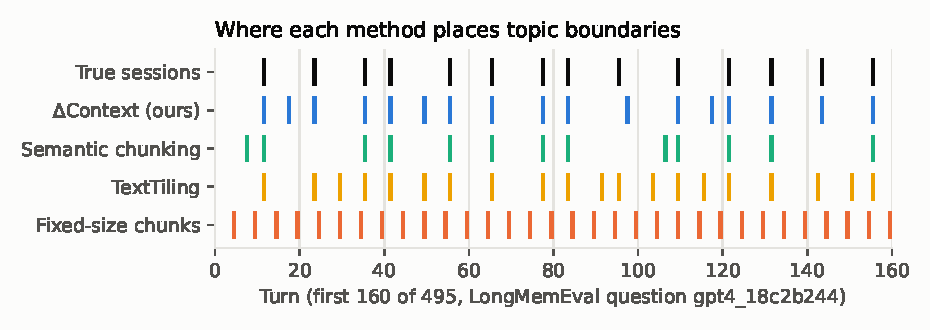
\includegraphics[width=\linewidth]{figures/segmentation_example.pdf}
\caption{Boundaries placed by each method on the first LongMemEval-S test
history (not selected), first 160 turns.}
\label{fig:example}
\end{figure}

Table~\ref{tab:seg} shows that \dc{} is the most accurate segmenter on every
metric: Pk 0.099 against 0.125 for the next best (the adjacent-turn threshold)
and boundary F1 0.840 against at most 0.778 (+0.062, 95\% CI [+0.054, +0.070]).
It decides boundaries online, whereas semantic chunking and TextTiling see the
whole history. Figure~\ref{fig:example} shows the typical pattern: \dc{}
matches nearly every session break with a few extra cuts, semantic chunking
misses several, TextTiling over-segments, and fixed chunks ignore content.

\paragraph{Ablations.} Both design choices are necessary. Without boundary
localisation, checkpoints land two turns after the switch and exact-boundary
F1 falls from 0.828 to 0.035; the path-length detector reaches only 0.208 F1
at $\pm1$. The same pattern holds downstream (Table~\ref{tab:ablation}): topic
hit@1 drops from 0.749 to 0.426 without localisation and to 0.640 with the
path-length detector (both $p < 0.001$).

\begin{table}[t]
\centering\small
\begin{tabular}{lrrr}
\toprule
Method & hit@1 & hit@3 & topic_recall \\
\midrule
\textbf{$\Delta$Context store (top-3)} & 0.749 & 0.917 & 0.716 \\
$\Delta$Context store (top-3) (no localization) & 0.426$^{*}$$^{*}$$^{*}$ & 0.732$^{*}$$^{*}$$^{*}$ & 0.516$^{*}$$^{*}$$^{*}$ \\
$\Delta$Context store (top-3) (path-length detector) & 0.640$^{*}$$^{*}$$^{*}$ & 0.847$^{*}$$^{*}$$^{*}$ & 0.609$^{*}$$^{*}$$^{*}$ \\
\bottomrule
\end{tabular}

\caption{Ablating \dc{} in the topic store (LongMemEval-S, budget 2048,
top-3 topics). Stars: significant difference from full \dc{}.}
\label{tab:ablation}
\end{table}

\subsection{Topic-structured store}
\label{sec:store}

\begin{table}[t]
\centering\small
\begin{tabular}{lrrrrr}
\toprule
Method & Hit@1 & Hit@3 & Topic rec. & Evid. rec. & Searched (\%) \\
\midrule
\textbf{$\Delta$Context topic store (ours)} & 0.770 & 0.930 & 0.732 & 0.733 & 17.1 \\
Session oracle topic store & 0.785 & 0.926 & 0.733 & 0.734 & 16.5 \\
Adjacent threshold topic store & 0.736 & 0.902 & 0.711 & 0.725 & 20.1 \\
Semantic chunking topic store & 0.721 & 0.904 & 0.704 & 0.717 & 18.4 \\
TextTiling topic store & 0.777 & 0.921 & 0.729 & 0.732 & 16.9 \\
Fixed-size chunks (5 turns) topic store & 0.457$^{***}$ & 0.736$^{***}$ & 0.534$^{***}$ & 0.581$^{***}$ & 23.1 \\
Fixed-size chunks (10 turns) topic store & 0.543$^{***}$ & 0.813$^{***}$ & 0.601$^{***}$ & 0.601$^{***}$ & 16.2 \\
RAG, full scan (turn-level) & -- & -- & 0.774$^{***}$ & 0.774$^{***}$ & 100.0 \\
\bottomrule
\end{tabular}

\caption{Topic-first stores on LongMemEval-S (budget 2048 tokens, top-3
topics, 470 answerable questions with evidence). Stars mark a significant
difference from \dc{} (Holm-adjusted; $^{*}p<.05$, $^{**}p<.01$,
$^{***}p<.001$). The last row searches every turn.}
\label{tab:store}
\end{table}

\begin{figure}[t]
\centering
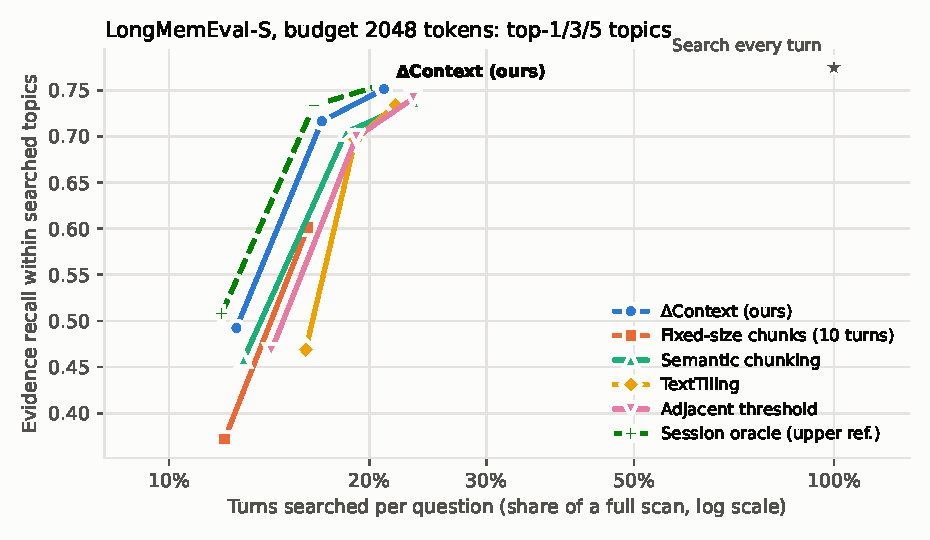
\includegraphics[width=0.49\linewidth]{figures/cost_recall.pdf}\hfill
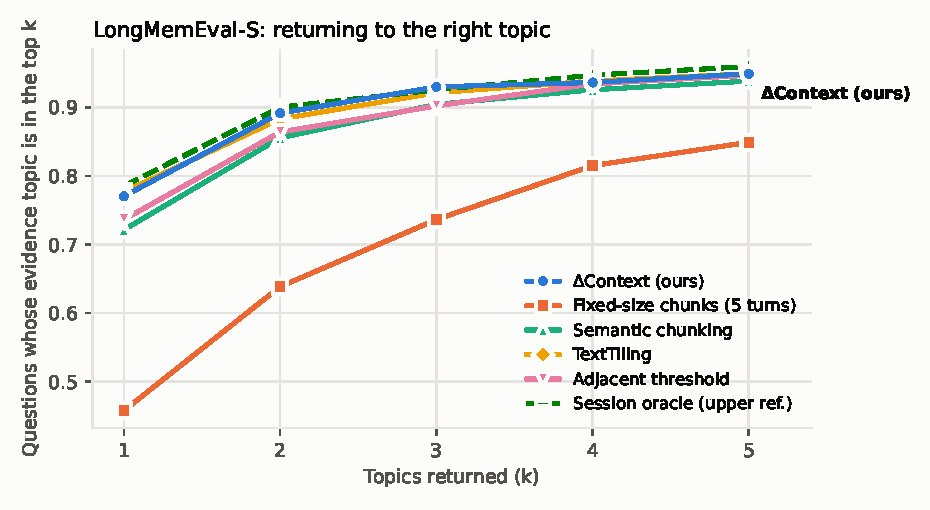
\includegraphics[width=0.49\linewidth]{figures/topic_hits.pdf}
\caption{LongMemEval-S topic stores. Left: share of a full scan searched vs.\
evidence recall within the searched topics, for the top 1, 3 and 5 topics.
Right: topic hit@$k$.}
\label{fig:store}
\end{figure}

Table~\ref{tab:store} and Figure~\ref{fig:store} evaluate the store on single
histories. Storing the chat as \dc{} segments returns the evidence's topic
first for 74.9\% of questions and within the top three for 91.7\%; searching
only those three topics (17\% of a full scan's comparisons) keeps 0.716 of the
evidence turns, 93\% of the 0.774 a full scan keeps ($-0.058$, CI
[$-0.079$, $-0.037$]). Semantic segmentation of any kind is far better than
fixed-size chunks (hit@1 +0.206 over 10-turn chunks, $p < 0.001$).

Among the semantic segmenters the differences are small. \dc{} is numerically
best at every $k$ and every cost point, closest to the session oracle, and
none of its 27 per-$k$ comparisons against semantic chunking, TextTiling and
the adjacent threshold is negative; but after correction only the gap to
TextTiling (mean hit@1--5, +0.029, $p = 0.016$) is significant. On a single
history of $\sim$48 topics, any reasonable semantic segmentation finds the
right topic most of the time.

\subsection{Scaling the store}
\label{sec:scaling}

\begin{table}[t]
\centering\small
\resizebox{\linewidth}{!}{\begin{tabular}{rccccccr}
\toprule
Turns & $\Delta$Ctx & Fixed & Semantic & TextTiling & Adjacent & Oracle & Comparisons ($\Delta$Ctx / full) \\
\midrule
492 & 0.78 / 0.92 & 0.59 / 0.84$^{**}$ & 0.72 / 0.92 & 0.78 / 0.92 & 0.74 / 0.90 & 0.79 / 0.92 & 84 / 492 \\
1,971 & 0.59 / 0.83 & 0.44 / 0.70$^{***}$ & 0.55 / 0.79 & 0.58 / 0.82 & 0.56 / 0.81 & 0.58 / 0.84 & 227 / 1,971 \\
4,917 & 0.49 / 0.69 & 0.35 / 0.53$^{***}$ & 0.43 / 0.65 & 0.51 / 0.70 & 0.45 / 0.68 & 0.49 / 0.71 & 512 / 4,917 \\
9,883 & 0.42 / 0.61 & 0.35 / 0.50$^{**}$ & 0.33 / 0.53 & 0.44 / 0.62 & 0.40 / 0.58 & 0.45 / 0.62 & 990 / 9,883 \\
19,732 & 0.28 / 0.48 & 0.19 / 0.38 & 0.25 / 0.43 & 0.32 / 0.49 & 0.28 / 0.47 & 0.30 / 0.48 & 1,949 / 19,732 \\
\bottomrule
\end{tabular}
}
\caption{Topic hit@1 / hit@3 as the store grows: each test question's history
placed after $D \in \{0, 3, 9, 19, 39\}$ other histories ($\sim$238 questions).
Stars: exact McNemar on hit@3 vs.\ \dc{}, Holm-adjusted over all 50 tests in the
table. Last column: query-time comparisons of \dc{} vs.\ a full scan.}
\label{tab:scaling}
\end{table}

\begin{figure}[t]
\centering
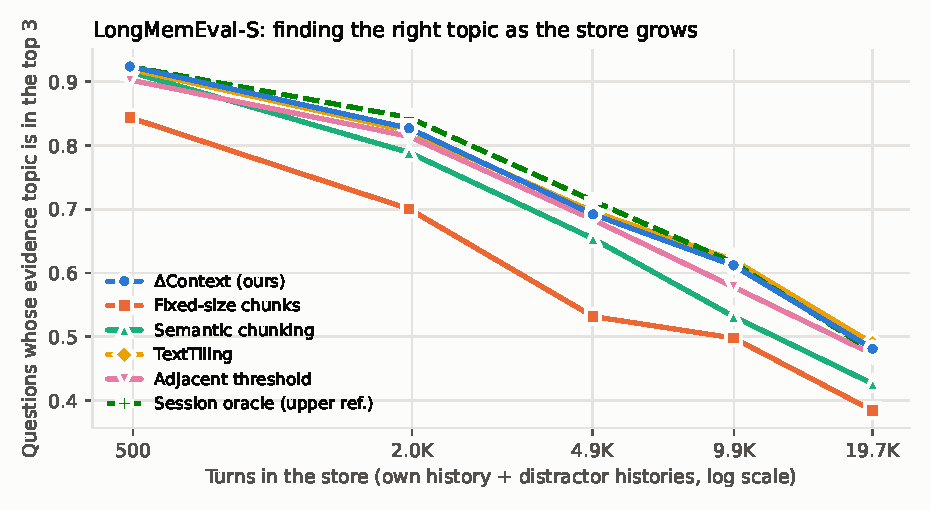
\includegraphics[width=0.75\linewidth]{figures/scaling.pdf}
\caption{Topic hit@3 as the store grows (log scale).}
\label{fig:scaling}
\end{figure}

A long-lived assistant's store holds far more than one history. We grow it by
placing each test question's history after $D$ other questions' histories
(Table~\ref{tab:scaling}, Figure~\ref{fig:scaling}). \dc{} stays within 1--3.3
points of the session oracle at every size while searching 11--17\% of the
store (10.5\% at $\sim$20K turns). Semantic chunking, whose percentile threshold is set over the whole
history, falls progressively behind: from $\sim$2K turns up its hit@1 trails
\dc{} by 0.08--0.10 (exact McNemar $p = 0.001$--$0.008$ per size before
correction; not significant after correcting over all 50 tests). Fixed chunks
lose significantly at every size. TextTiling matches \dc{}'s hit rates but is
offline and its segments cost 30--38\% more comparisons from $\sim$2K turns up.

\subsection{End-to-end question answering}
\label{sec:qa}

\begin{table}[t]
\centering\small
\begin{tabular}{lrrrrr}
\toprule
Method & f1 & em & evidence_recall & context_tokens & Abstain \\
\midrule
Sliding window & 0.026$^{*}$$^{*}$$^{*}$ & 0.006$^{*}$$^{*}$$^{*}$ & 0.011$^{*}$$^{*}$$^{*}$ & 482.629 & 0.975 \\
Extractive summary & 0.026$^{*}$$^{*}$$^{*}$ & 0.006$^{*}$$^{*}$$^{*}$ & 0.004$^{*}$$^{*}$$^{*}$ & 467.018 & 0.971 \\
RAG + recency tail (50/50) & 0.223 & 0.073 & 0.374 & 483.764 & 0.688 \\
RAG, turn-level & 0.259$^{*}$$^{*}$$^{*}$ & 0.081 & 0.475$^{*}$$^{*}$$^{*}$ & 506.748 & 0.646 \\
RAG + chunk prior & 0.267$^{*}$$^{*}$$^{*}$ & 0.086 & 0.494$^{*}$$^{*}$$^{*}$ & 506.640 & 0.614 \\
\textbf{$\Delta$Context turn ranking (v1.2)} & 0.228 & 0.075 & 0.375 & 485.936 & 0.673 \\
\bottomrule
\end{tabular}

\caption{LoCoMo QA with Qwen2.5-3B-Instruct, budget 512 tokens, 1,540
answerable probes (abstention rate on the 446 adversarial probes in the last
column). Stars: significant difference from \dc{}'s topic store
(Holm-adjusted).}
\label{tab:locomo-qa}
\end{table}

\begin{table}[t]
\centering\small
\begin{tabular}{lrrrrr}
\toprule
Method & F1 & EM & Evid. rec. & Tokens & Abstain \\
\midrule
\bottomrule
\end{tabular}

\caption{LongMemEval-S QA with Qwen2.5-3B-Instruct, budget 2048 tokens.
Stars: significant difference from \dc{}'s topic store (Holm-adjusted).
\pending{final runs in progress}}
\label{tab:lme-qa}
\end{table}

On LoCoMo (Table~\ref{tab:locomo-qa}), the corrected evaluation and a stronger
generator lift every retrieval policy far above truncation (F1 0.22--0.27 vs.\
0.03), and spending the whole budget on retrieved turns rather than splitting
it with a recency tail adds 0.036 F1. \dc{}'s topic store (0.220) is
statistically tied with the other topic stores and below a full scan (0.259,
$-0.039$, CI [$-0.052$, $-0.026$]). LoCoMo has no topic structure for the store
to exploit, and \dc{}'s LongMemEval-tuned threshold produces segments so large
that the top three cover about half of each conversation. On LongMemEval-S
(Table~\ref{tab:lme-qa}) \pending{results pending}.

% ---------------------------------------------------------------------------
\section{What Did Not Help}
\label{sec:negative}

\paragraph{Topic-first search does not beat a full scan on recall.} At equal
budget, scanning every turn keeps more evidence (0.774 vs.\ 0.716 on
LongMemEval-S) and answers LoCoMo better. The case for a topic store is cost
and structure, not recall.

\paragraph{Segments as a ranking prior.} Before treating segments as storage
units we used them as a prior in turn ranking, scoring each turn by its own
similarity plus a weighted similarity of its segment. On LoCoMo this added 2--3
points of evidence recall, but fixed-size chunks gave the same gain; on
LongMemEval-S no prior, including the oracle sessions, beat plain retrieval.

\paragraph{Topic state as a recency signal.} For questions asked right after
their evidence, a recency tail helps at large budgets (LoCoMo, budget 2048:
0.923 vs.\ 0.802 evidence recall), so the right budget split depends on the
question. Whether the best-matching turn is recent separates these questions
far better (AUC 0.85) than the question's similarity to \dc{}'s current topic
(AUC 0.63).

\paragraph{Earlier evaluation.} Under the uncorrected LoCoMo setup with a 1.1B
model, every policy scored F1 0.06--0.12 and a query-aware \dc{} variant
appeared to match retrieval exactly; it was in fact ranking the same turns,
answering 1,214 of 1,986 probes identically.

% ---------------------------------------------------------------------------
\section{Limitations}

LongMemEval's official metric is an LLM judge; we report token F1, exact match
and evidence recall, which favour short exact answers. We use one generator
size and one small embedder; absolute QA scores would rise with larger models.
The scaling study grows stores with other users' histories, which are more
distinct from one another than a single user's long-lived chat would be.
LoCoMo, a dialogue between two people over months, is not a topic-segmentation
benchmark, and our LoCoMo store results are confounded by segment granularity.
Questions within a LoCoMo conversation are not independent, so LoCoMo
$p$-values are likely optimistic. All experiments ran on a single 8\,GB GPU.

% ---------------------------------------------------------------------------
\section{Conclusion}

Storing a conversation as topic segments found online is a practical way to
organise long-term chat memory. \dc{}'s displacement detector with boundary
localisation segments conversations more accurately than offline semantic
chunking and TextTiling, and a store built on it finds the right topic for most
questions while searching an order of magnitude fewer items than a full scan,
staying close to oracle segmentation as the store grows. It does not replace a
full scan when recall is all that matters. We release \textsc{ContextBench}, the
corrected LoCoMo scoring, and all scripts that regenerate these tables and
figures from run outputs.

\bibliographystyle{plainnat}
\bibliography{references}

\end{document}
